\section{Results}
\label{sec:analysis}

The keyword solution and modifications to fission as described in subsections ~\ref{sec:desugar} and ~\ref{sec:fission} was implemented into the StreamIt compiler.  The sample benchmarks in Figure~\ref{fig:theo-speedups} were rewritten to use the {\tt iter()} keyword, allowing the compiler to expose data parallelism in its stream graph.


\subsection{FIRBankPipeline}
\begin{figure}[t]
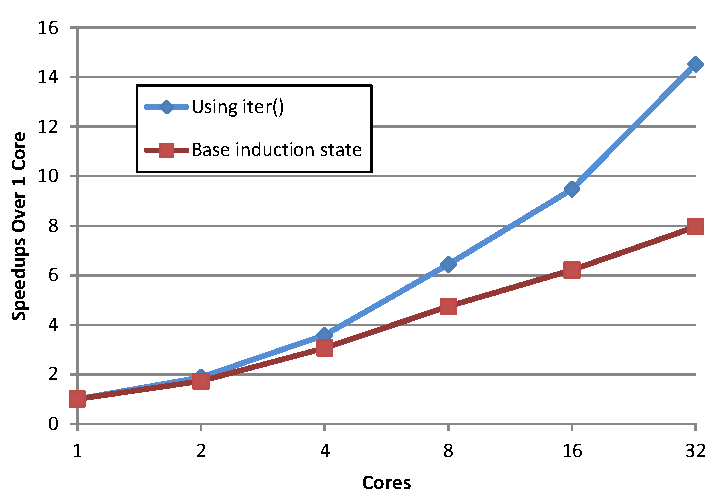
\includegraphics[width=3.3in]{figures/firbank-results.pdf}
\caption{Speedups for FIRBankPipeline, with and without induction variable state.  \protect\label{fig:firbank-results}}
\end{figure}

FIRBankPipeline contains one filter that uses induction variable state with 3.94\% of program's work.  This filter, Multiply, maintains induction state in an index that traces through the rows of a two dimensional array.  Each invocation performs complex multiplication on the stream input values and the array elements of that specified row.  

Figure~\ref{fig:firbank-results} indicates the speedups over 1 core for both induction state and iteration keyword implementations.  Between the two implementations, there is 1.38X speedup on 8 cores, 1.55X speedup on 16 cores, and 1.85X speedup on 32 cores for the iteration keyword implementation.  This abides fairly closely with the model as described in Section ~\ref{sec:model-analysis}.  